\section{Introduction}
Databases are susceptible to various forms of corruption, or \emph{dirtiness}, such as missing, incorrect, or inconsistent values.
Numerous industrial surveys have shown that dirty data are prevalent \cite{Gartner}, and there is now a growing industry around cleaning data at scale \cite{fortunearticle}.
One reasons for the recent research and commercial interest in data cleaning is analysts are increasingly deriving data from inherently error-prone processes such as extracting structured data from websites, synthesizing data from multiple networked sensors, and linking entities from disparate data sources.
New methodologies for scalable and reliable analysis in the presence of errors are required. 

The analysis performed on the data is also becoming more complex.
The endpoint of modern data analysis pipelines can be any number of ``data products", such as recommender systems, spam detectors, and forecasting models, all of which can be very sensitive to data quality \cite{xiaofeature}.
Increasingly, analytics stacks are moving beyond traditional SQL analytics and natively supporting Machine Learning (e.g. Berkeley Data Analytics Stack \cite{bdas}, Hadoop, Stratosphere \cite{alexandrov2014stratosphere}).
When error is systematic, i.e., correlated with the data, errors can significantly bias predictions by a model.
For example, in a recommender system, we may find that all users from one region have a missing age attribute.
Discarding or ignoring this problem can make predictions for the affected subpopulation untrustworthy.
While there is an extensive literature on robust Machine Learning, this work largely focuses on resilience to atypical outliers and not systematically corrupted data.

Since new analytics frameworks encapsulate the entire data processing pipeline from raw data to features to model training, there is an opportunity to address this problem from database perspective.  
The database community's response to systematic corruption is data cleaning, which is an extensively studied field (see Rahm and Do \cite{rahm2000data} for a survey).
Cleaning works by repairing (or approximately repairing) the corruption in the base data.
However, cleaning large data can be expensive, both computationally and in human effort, as an analyst has to program repairs for all errors manifest in the data \cite{kandel2012}.
In some applications, scripted data transformations may not be reliable necessitating the use of even costlier crowdsourcing techniques \cite{gokhale2014corleone,park2014crowdfill}.

An emerging solution to the growing costs of data cleaning is sampling \cite{wang1999sample}, where the analyst cleans a small sample of data and can estimate the results of aggregate queries.
Analysts can sample a large dataset, prototype changes on the sample, and evaluate whether these changes have the desired affect.
Sampling provides a flexible tradeoff between cleaning cost and query result accuracy for aggregate queries.
The case for sampling in data cleaning is analogous to arguments for Approximate Query Processing (AQP) \cite{DBLP:conf/eurosys/AgarwalMPMMS13}, where a timely approximate answer is more desirable than an exact slow answer. 

\begin{figure}[t]
\centering
 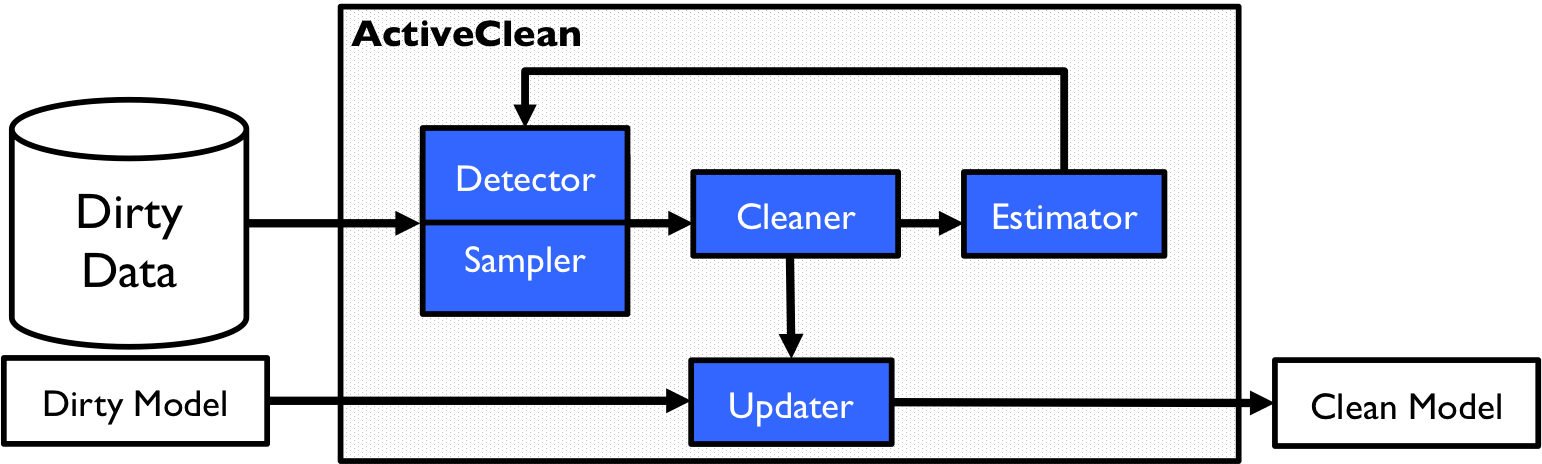
\includegraphics[width=0.8\columnwidth]{figs/arch.png}
 \caption{\sysfull presents an adaptive architecture for iteratively correcting dirty Machine Learning models. Users specific error detection and repair procedures and the framework will iteratively clean and sample batches of data from which it will update the model. The detection can be adaptive learning from the repairs. \label{sys-arch}}\vspace{-2em}
\end{figure}

Unfortunately, a naive application of sampling does not generalize to Machine Learning.
Machine Learning is far more sensitive to sample size (training data) than aggregate queries.
Suppose we have a budget of cleaning only 50 records.
This might be sufficient data to approximate some basic aggregate queries such sums and counts, but in any moderately difficult Machine Learning application, 50 examples is not sufficient to train an accurate model.
In other words, in small samples, the error mitigation by data cleaning is dominated by the error introduced by sampling.

In this work, we explore better methodologies for training models under budgeted data cleaning.
One insight is that errors are often sparse and affect a small number of examples and features.
This means that a model trained on the full dirty data may be relatively ``close" to the true clean model.
So instead of attempting to retrain a model from scratch, we can try to correct the old model.
The next insight that errors often happen in batches, i.e., there are groups of similarly corrupted records, and as we clean more data, we get more information about how groups of errors affect the model.
Instead of cleaning a sample of data all at once, we should be cleaning small batches and feeding that information back to inform subsequent iterations.

In this paper, we propose \sys, an anytime framework for training Machine Learning models with budgeted data cleaning (Figure \ref{sys-arch}).
Users of \sys have to initialize with a dirty model, and specify an error detection procedure and an error repair method.
Our system will provide a framework to return an accurate model given a repair budget.
\sys partitions the dirty and clean data, samples from the dirty data, applies the repairs, then updates the model.
After model update, the repairs are fed back into the sampling stage to adaptively select the data that are most valuable to our model.
We can also update the error detection procedure based on our observations in the sample.
\sys supports a broad class of models which includes linear regression, logistic regression, generalized linear models, and support vector machines.

\sys presents a novel framework that tightly integrates data cleaning with model training.
As a result, there are numerous new opportunities for optimization.
We can ``push down" the model training to the data cleaning and select data to clean that are most valuable to the model.
We can also ``push up" the data cleaning to the model training by intelligently batching together model updates on already cleaned data.
In summary, our contributions are
\begin{itemize}[noitemsep]
\item We propose \sysfull which given dirty data, a model, a data cleaning procedure, and a budget, we can return a highly accurate model for a fraction of the cleaning cost.
\item \sys proposes a novel framework that iteratively corrects a model based on small batches of clean data.
\item \sys relies on two key optimizations, guided error sampling and error partitioning, that result in substantial empirical gains in accuracy in comparison to alternative approaches such as Active Learning.
\item We evaluate \sysfull on real and synthetic datasets to show that non-uniform sampling achieves improved performance in comparison to uniform sampling, and Active Learning.
\end{itemize}








